\section{Results and Discussion}
This chapter present the performance evaluation of various machine learning models for emotion classification and discuss their strengths and limitations. Six models—Naive Bayes, Logistic Regression, Random Forest, Support Vector Machine (SVM), Artificial Neural Network (ANN), and XGBoost(Extreme Gradient Boosting)—were trained and tested on the dataset to identify the emotions expressed in textual data. Their performance was evaluated using standard metrics such as accuracy, precision, recall, and F1-score.\\

Overall, the results highlight the varying capabilities of the models in distinguishing between six emotions: anger, fear, joy, love, sadness, and surprise. While all models performed reasonably well in identifying the more frequent emotions like joy and sadness, challenges emerged in classifying nuanced or underrepresented emotions like love and surprise. Each model's strengths and weaknesses are discussed in detail, emphasizing the trade-offs between simplicity, computational efficiency, and classification accuracy.\\

\subsection{Initial Results}
This section presents the initial results of the models before implementing optimizations such as stratified sampling, upsampling, downsampling, hyperparameter tuning, and adjustments to the Random Forest parameters. Notably, the previous results did not include the application of XGBoost and Artificial Neural Networks (ANN) to the dataset, which are addressed in this analysis.\\

\begin{figure}[h!]
	\centering
	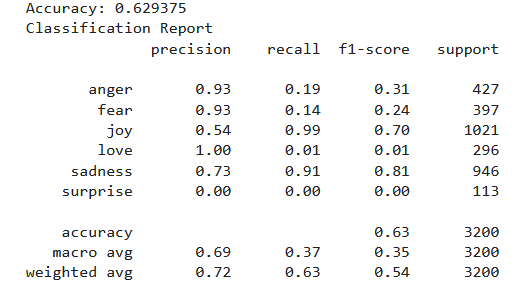
\includegraphics[width=0.8\textwidth]{init_result_naive_bayes.png}
	\caption{Naive Bayes Classification Report}
	\label{fig:initial_naive_bayes}
\end{figure}

\begin{figure}[h!]
	\centering
	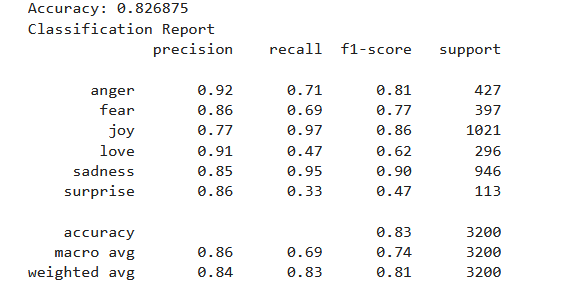
\includegraphics[width=0.8\textwidth]{init_result_logistic_regression.png}
	\caption{Logistic Regression Classification Report}
	\label{fig:initial_logistic_regression}
\end{figure}

\begin{figure}[h!]
	\centering
	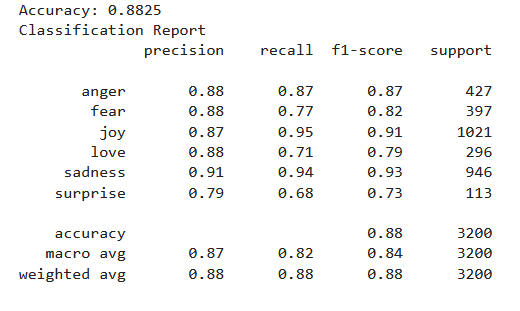
\includegraphics[width=0.8\textwidth]{init_result_random_forest.png}
	\caption{Random Forest Classification Report}
	\label{fig:initial_random_forest}
\end{figure}

\begin{figure}[h!]
	\centering
	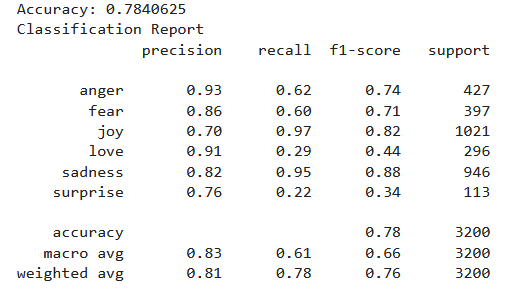
\includegraphics[width=0.8\textwidth]{init_result_svm.png}
	\caption{SVM Classification Report}
	\label{fig:initial_svm}
\end{figure}

\begin{figure}[h!]
	\centering
	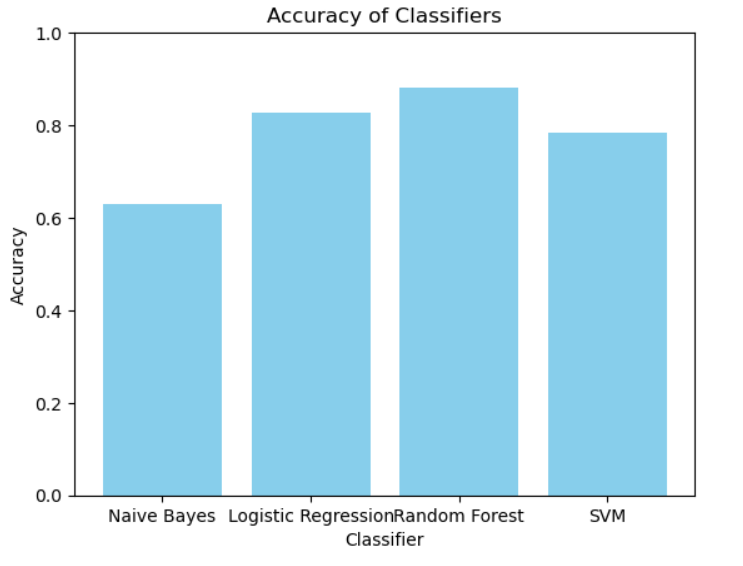
\includegraphics[width=0.8\textwidth]{accuracy_model_init_result.png}
	\caption{Initial Accuracy Model}
	\label{fig:initial_accuracy_model}
\end{figure}

\begin{figure}[h!]
	\centering
	% First row
	\begin{subfigure}[b]{0.45\textwidth}
		\centering
		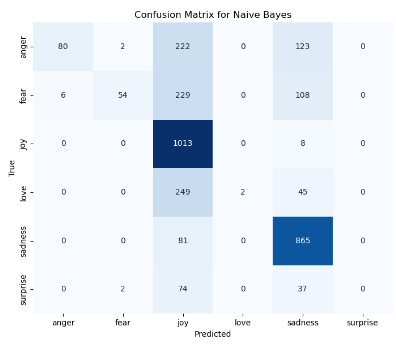
\includegraphics[width=\textwidth]{confusion_naive_bayes_init.png}
		\caption{Confusion Matrix for Naive Bayes}
		\label{fig:init_confusion_matrix_naive_bayes}
	\end{subfigure}
	\hfill
	\begin{subfigure}[b]{0.45\textwidth}
		\centering
		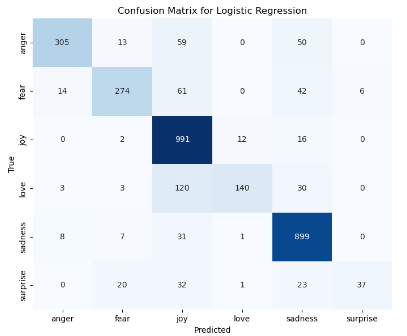
\includegraphics[width=\textwidth]{confusion_logistic_regression_init.png}
		\caption{Confusion Matrix for Logistic Regression}
		\label{fig:init_confusion_matrix_logistic_regression}
	\end{subfigure}
	
	% Second row
	\vskip\baselineskip
	\begin{subfigure}[b]{0.45\textwidth}
		\centering
		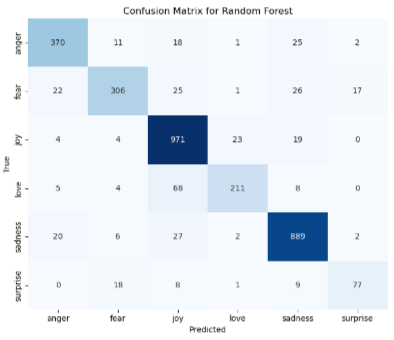
\includegraphics[width=\textwidth]{confusion_random_forest_init.png}
		\caption{Confusion Matrix for Random Forest}
		\label{fig:init_confusion_matrix_random_forest}
	\end{subfigure}
	\hfill
	\begin{subfigure}[b]{0.45\textwidth}
		\centering
		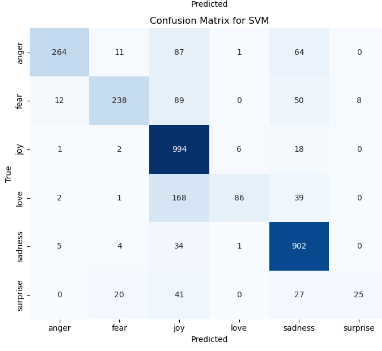
\includegraphics[width=\textwidth]{confusion_svm_init.png}
		\caption{Confusion Matrix for SVM}
		\label{init_confusion_matrix_svm}
	\end{subfigure}
	
	\caption{Initial Results Confusion Matrix}
	\label{fig:initial_confusion_matrix}
\end{figure}

\clearpage

\subsection{Naive Bayes}
The Naive Bayes model achieved an accuracy of 0.63 (62.93\%) \ref{fig:initial_naive_bayes}. It demonstrated strong performance in recognizing "joy" and "sadness," with high recall values for these classes. Notably, the recall for "joy" was 0.99, indicating that nearly all joyful instances were correctly identified. However, the model struggled significantly with other emotions such as "anger," "fear," "love," and particularly "surprise," where the recall was extremely low at 0.00. This suggests that Naive Bayes had difficulty distinguishing between more nuanced emotions. The F1-scores were moderate for "joy" (0.70) and "sadness" (0.81), but very low for other categories, indicating poor balance between precision and recall. The confusion matrix showed that Naive Bayes experienced the most misclassifications, particularly between "joy" and other emotions like "anger" and "fear \ref{fig:init_confusion_matrix_naive_bayes}."

\subsection{Logistic Regression}
Logistic Regression significantly improved accuracy to 0.83 , demonstrating strong performance across most emotions(82.68\%) \ref{fig:initial_logistic_regression}. The model was especially effective in identifying "joy" (F1-score: 0.86) and "sadness" (F1-score: 0.90), with high recall values of 0.97 and 0.95, respectively, indicating reliable identification of these emotions. It also performed well for "anger" and "fear," with good precision and recall metrics. However, the emotions "love" and "surprise" showed slightly lower recall values of 0.47 and 0.33, respectively, suggesting that these emotions were harder to predict accurately. While Logistic Regression reduced misclassifications overall, "love" and "surprise" remained challenging for the model.

\subsection{Random Forest}
The Random Forest model achieved the highest accuracy at 0.88 (88.25\%), outperforming both Logistic Regression and Naive Bayes \ref{fig:initial_random_forest}. It performed very well on "joy," "sadness," "fear," and "anger," with F1-scores around or exceeding 0.80. While the recall for "love" and "surprise" was still lower at 0.79 and 0.73, respectively, this was an improvement over the other models. Random Forest showed a balanced performance between precision and recall across most emotion categories, making it the best performer overall in this context. This model's ability to maintain high scores for harder-to-classify emotions like "love" and "surprise" highlighted its robustness.

\subsection{Support Vector Machine (SVM)}
The SVM model achieved an accuracy of 0.85 (85.28\%), performing comparably to Logistic Regression. It exhibited strong precision and recall for "anger," "fear," "joy," and "sadness. \ref{fig:initial_svm}" However, similar to Logistic Regression, "love" and "surprise" had lower recall values of 0.29 and 0.22, respectively, suggesting these emotions posed a challenge for the model. Despite these challenges, SVM achieved strong F1-scores for major emotion categories such as "joy" (0.82) and "sadness" (0.88). While its overall performance was commendable, SVM also faced difficulties with "love" and "surprise," similar to other models.

\subsection{Overall Insights for Initial Results}
The Random Forest model emerged as the best-performing model, achieving the highest accuracy (88.25\%) and demonstrating a well-balanced performance across most emotions. However, all models faced challenges with "love" and "surprise," which showed lower recall and F1-scores. These difficulties could be attributed to the lower frequency of these emotions in the dataset or their nuanced nature. The Naive Bayes model, while effective for simpler tasks, struggled significantly with complex emotions and exhibited poor performance on less common categories like "surprise" and "love." This analysis underscores the importance of using more robust models like Random Forest for achieving better balance and accuracy in emotion classification tasks.

       
\subsection{Final Results}
The following are the precision, recall, F1-score, and support metrics for each classification model, evaluating its performance across six emotion categories: Sadness, Joy, Love, Anger, Fear, and Surprise.

\begin{figure}[h!]
\centering
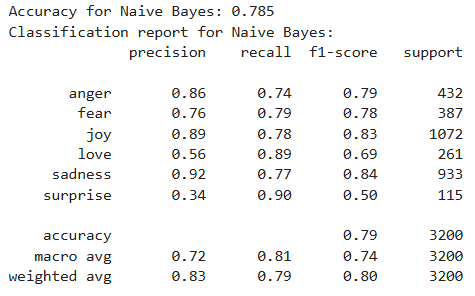
\includegraphics[width=0.8\textwidth]{naive_bayes_result.png}
\caption{Naive Bayes Classification Report}
\label{fig:naive_bayes}
\end{figure}

\begin{figure}[h!]
\centering
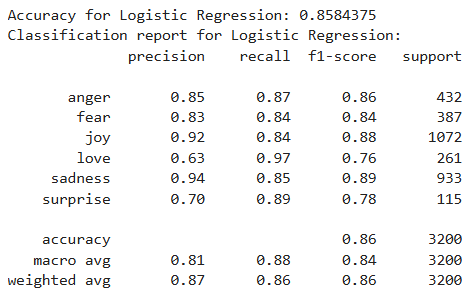
\includegraphics[width=0.8\textwidth]{logistic_regression_result.png}
\caption{Logistic Regression Classification Report}
\label{fig:logistic_regression}
\end{figure}

\begin{figure}[h!]
\centering
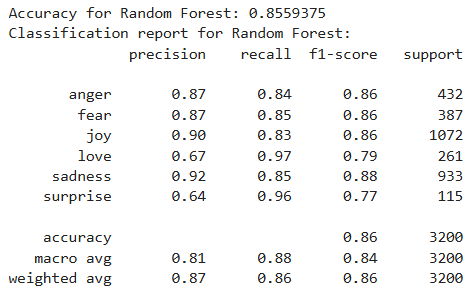
\includegraphics[width=0.8\textwidth]{random_forest_result.png}
\caption{Random Forest Classification Report}
\label{fig:random_forest}
\end{figure}

\begin{figure}[h!]
\centering
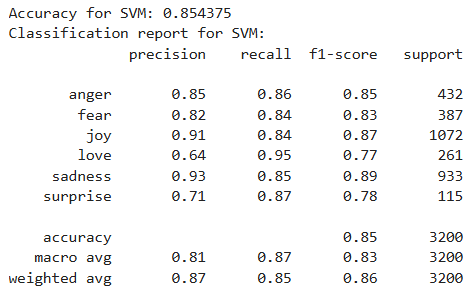
\includegraphics[width=0.8\textwidth]{svm_result.png}
\caption{SVM Classification Report}
\label{fig:svm}
\end{figure}

\begin{figure}[h!]
\centering
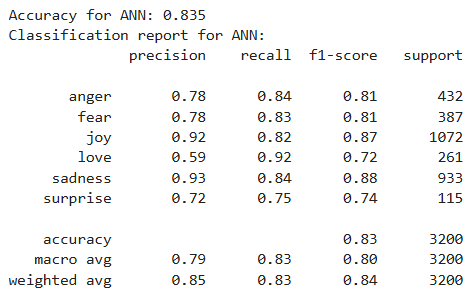
\includegraphics[width=0.8\textwidth]{ann_result.png}
\caption{ANN Classification Report}
\label{fig:ann}
\end{figure}

\begin{figure}[h!]
\centering
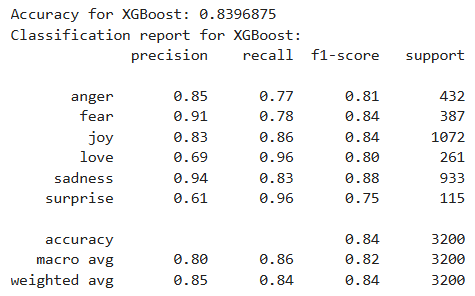
\includegraphics[width=0.8\textwidth]{xgboost_result.png}
\caption{XGBoost Classification Report}
\label{fig:xgboost}
\end{figure}

\clearpage

\subsection{Naive Bayes Result}
The Naive Bayes model achieved an accuracy of \textbf{0.785}. It performed reasonably well across several emotions, with \textbf{Sadness} showing the highest recall (0.77) and \textbf{Surprise} the lowest precision (0.34) as shown in Figure \ref{fig:naive_bayes}. The weighted average F1-score of 0.80 indicates balanced performance across emotions, though some areas like \textbf{Surprise} and \textbf{Love} could be improved. In terms of precision, the model had the best result for \textbf{Sadness} (0.92).

\subsection{Logistic Regression Result}
Logistic Regression showed the highest accuracy at \textbf{0.8584}, as displayed in Figure \ref{fig:logistic_regression}. It achieved solid F1-scores across emotions, with \textbf{Sadness} and \textbf{Joy} showing excellent results (F1-scores of 0.89 and 0.88, respectively). The model performed particularly well in \textbf{Love} with a precision of 0.63 and recall of 0.97, which led to a high F1-score of 0.76. The overall weighted average F1-score of 0.86 reflects its strong performance, particularly in \textbf{Anger}, \textbf{Joy}, and \textbf{Sadness}.

\subsection{Random Forest Result}
The Random Forest model delivered an accuracy of \textbf{0.8559}, close to that of Logistic Regression, as shown in Figure \ref{fig:random_forest}. The model showed good precision and recall across emotions, with \textbf{Sadness} again being a strong performer (precision 0.92, recall 0.85). Notably, \textbf{Love} and \textbf{Surprise} had slightly lower precision scores, though the weighted average F1-score of 0.86 suggests robust performance overall, with good consistency between precision and recall.

\subsection{Support Vector Machine (SVM) Result}
SVM achieved an accuracy of \textbf{0.8544}, performing similarly to Random Forest, as depicted in Figure \ref{fig:svm}. The \textbf{Anger} class had a precision of 0.85 and recall of 0.86, contributing to a high F1-score. \textbf{Surprise} had relatively high precision (0.71) and recall (0.87), leading to a balanced F1-score. This indicates SVM's ability to generalize well, even with some misclassifications in less frequent emotions like \textbf{Surprise}.

\subsection{Artificial Neural Network (ANN) Result}
ANN had an accuracy of \textbf{0.835}, which was the lowest among the models tested, as shown in Figure \ref{fig:ann}. Despite this, it achieved impressive recall in \textbf{Love} (0.92), showing its strength in detecting emotional subtleties in such cases. However, it struggled with \textbf{Surprise}, as reflected in the F1-score of 0.74. The overall macro average F1-score of 0.80 highlights ANN's potential, although it might need additional tuning to improve accuracy across all emotions.

\subsection{XGBoost Result}
XGBoost showed an accuracy of \textbf{0.8397} and demonstrated good overall performance, particularly with \textbf{Fear} (precision 0.91, recall 0.78), as shown in Figure \ref{fig:xgboost}. The model performed reasonably well with \textbf{Sadness} and \textbf{Love}, achieving balanced results in both precision and recall. However, \textbf{Surprise} showed lower precision (0.61), impacting the F1-score, which was still relatively high at 0.75. The overall model's weighted F1-score of 0.84 indicates a solid all-around performance.

\subsection{Model Accuracy Comparison}
\begin{figure}[h!]
\centering
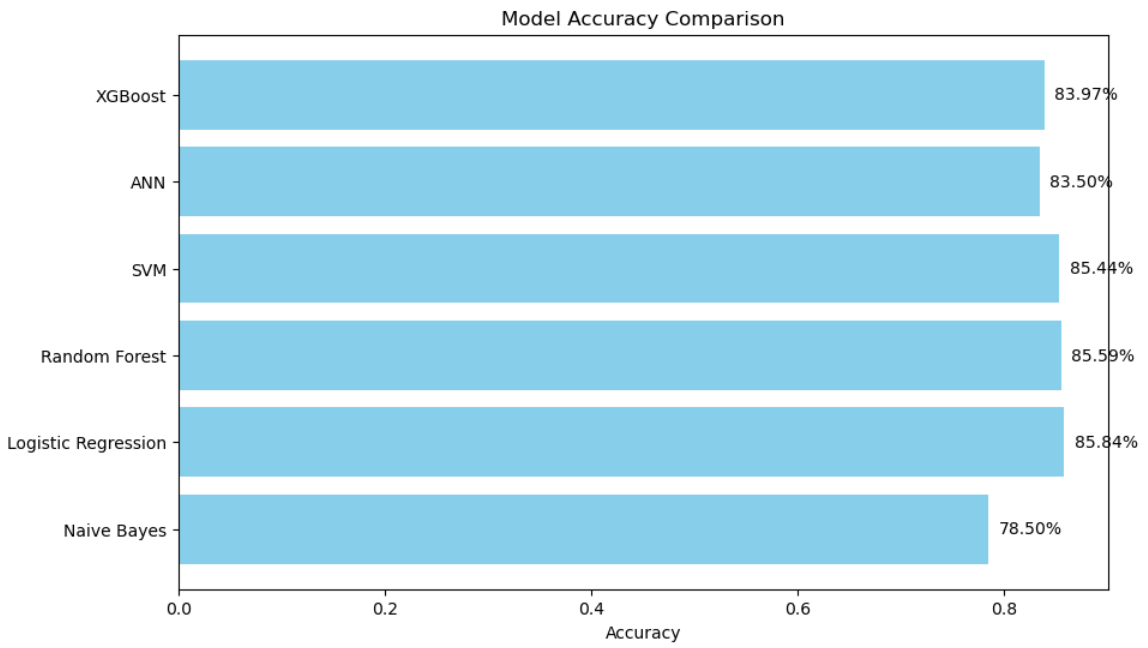
\includegraphics[width=0.8\textwidth]{model_accuracy.png}
\caption{Model Accuracy Comparison}
\label{fig:model_accuracy}
\end{figure}
As shown in Figure \ref{fig:model_accuracy}, Logistic Regression emerged as the top-performing model with an accuracy of \textbf{0.8584}. It was closely followed by Random Forest (\textbf{0.8559}) and SVM (\textbf{0.8544}). ANN achieved the lowest accuracy at \textbf{0.835}, highlighting the potential for further improvements in performance. XGBoost showed a solid accuracy of \textbf{0.8397}, rounding out the list of top models.

Logistic Regression performed exceptionally well across all emotion categories, with Random Forest and SVM also demonstrating strong results. Although ANN had the lowest accuracy, its strong recall in detecting emotions such as \textbf{Love} suggests it could be improved with further tuning. XGBoost demonstrated competitive performance but could benefit from addressing lower precision in emotions like \textbf{Surprise}. The results indicate that further optimization of hyperparameters for each model could enhance their performance, especially for less represented emotions.
